% Propietario conservado: /Users/ruben/Documents/New project/output/REVISION_ARGUMENTAL_APERTURAS_CIERRES_20260915/VI/delivery/MANUSCRIPT_VI_ES_EN_COMPLETE/source_es/sections/04_atlas_familias.tex
\section{Clasificación de las secciones persistentes y de sus observables internos}
\label{vi:vi:sec:atlas}

La clasificación comienza en el soporte sobre el que actúa el transporte.
Los nombres físicos se interpretan después de construir sus invariantes.
Esta prioridad permite distinguir una posición, una historia y una especie:
la posición pertenece al atlas finito; la historia conserva las transiciones
que la producen; el tipo de persistencia reúne historias compatibles con una
misma clasificación. Una masa evaluada es una lectura posterior de ese objeto.

\subsection{Paridad, profundidad y multisecciones}

Sobre la copia posicional de APP se considera
\[
 I_9=\{1,\ldots,9\},\qquad \mathcal C=I_9\times I_9.
\]
La pareja ordenada conserva los dos ejes. Definimos el clasificador de paridad
\[
 f(r,c)=
 \begin{cases}
 \ell,&r,c\text{ impares},\\
 \nu,&r\text{ impar},\ c\text{ par},\\
 d,&r\text{ par},\ c\text{ impar},\\
 u,&r,c\text{ pares},
 \end{cases}
 \qquad g(r,c)=\max\{|r-5|,|c-5|\}.
\]
Los símbolos de la primera aplicación nombran inicialmente clases internas.
La segunda mide profundidad combinatoria respecto del centro. La asociación
posterior con sectores físicos debe conservar estas definiciones.


% BEGIN OWNER /Users/ruben/Documents/New project/output/REVISION_ARGUMENTAL_APERTURAS_CIERRES_20260915/VI/delivery/MANUSCRIPT_VI_ES_EN_COMPLETE/source_es/figures/atlas_clasificacion.tex
\begin{figure}[H]
\centering
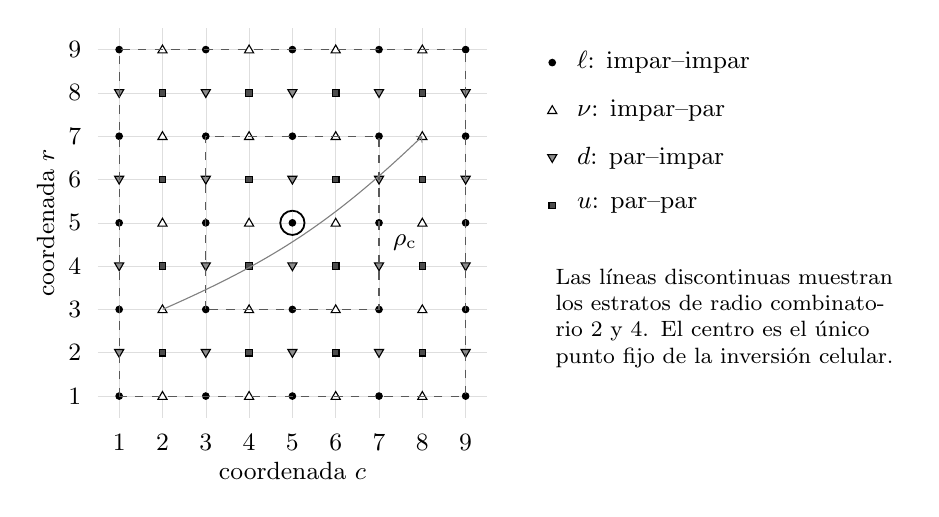
\begin{tikzpicture}[x=.55cm,y=.55cm, every node/.style={font=\small}]
  \draw[step=1,black!13,very thin] (.5,.5) grid (9.5,9.5);
  \foreach \k in {1,...,9} {
    \node[below] at (\k,.35) {$\k$};
    \node[left] at (.35,\k) {$\k$};
  }
  \node[below] at (5,-.3) {coordenada $c$};
  \node[rotate=90] at (-.7,5) {coordenada $r$};
  \foreach \r in {1,...,9} {
    \foreach \c in {1,...,9} {
      \pgfmathtruncatemacro{\pr}{mod(\r,2)}
      \pgfmathtruncatemacro{\pc}{mod(\c,2)}
      \ifnum\pr=1
        \ifnum\pc=1
          \draw[fill=black] (\c,\r) circle (.075);
        \else
          \draw[fill=white] (\c,\r+.105)--(\c-.105,\r-.075)--(\c+.105,\r-.075)--cycle;
        \fi
      \else
        \ifnum\pc=1
          \draw[fill=black!45] (\c,\r-.105)--(\c-.105,\r+.075)--(\c+.105,\r+.075)--cycle;
        \else
          \draw[fill=black!70] (\c-.075,\r-.075) rectangle (\c+.075,\r+.075);
        \fi
      \fi
    }
  }
  \draw[black!65,dashed] (3,3) rectangle (7,7);
  \draw[black!65,dashed] (1,1) rectangle (9,9);
  \draw[line width=.65pt] (5,5) circle (.28);
  \draw[->,black!50] (2,3) to[bend right=10] (8,7);
  \node[fill=white,inner sep=2pt] at (7.6,4.55) {$\rho_{\mathrm c}$};
  \begin{scope}[shift={(11,8.7)}]
    \draw[fill=black] (0,0) circle (.075);
    \node[right] at (.35,0) {$\ell$: impar--impar};
    \draw[fill=white] (0,-.995)--(-.105,-1.175)--(.105,-1.175)--cycle;
    \node[right] at (.35,-1.1) {$\nu$: impar--par};
    \draw[fill=black!45] (0,-2.305)--(-.105,-2.125)--(.105,-2.125)--cycle;
    \node[right] at (.35,-2.2) {$d$: par--impar};
    \draw[fill=black!70] (-.075,-3.375) rectangle (.075,-3.225);
    \node[right] at (.35,-3.3) {$u$: par--par};
    \node[anchor=west,text width=4.4cm,align=left,font=\footnotesize]
      at (-.15,-5.9) {Las líneas discontinuas muestran los estratos de radio combinatorio $2$ y $4$. El centro es el único punto fijo de la inversión celular.};
  \end{scope}
\end{tikzpicture}
\caption[Clasificación sobre el atlas posicional]{Clasificación sobre el atlas posicional. Las marcas distinguen las
cuatro clases internas de paridad, anteriores a sus realizaciones físicas.
La profundidad se mide con $g(r,c)=\max(|r-5|,|c-5|)$.
La flecha ilustra $(2,3)\mapsto(8,7)$ bajo la inversión celular;
no representa una trayectoria dinámica ni un cambio de sabor.
El círculo central marca $(5,5)$, de profundidad cero.}
\label{vi:vi:fig:atlas}
\end{figure}

% END OWNER


\begin{definition}[Multisección de familia y profundidad]
Para cada pareja realizada \(y=(f,g)\), se define
\[
 \mathfrak S_y=\{(r,c)\in\mathcal C:(f(r,c),g(r,c))=y\}.
\]
Su elevación a los estados persistentes es la preimagen por la proyección
al atlas, conservando las hojas, las orientaciones y la memoria de la extensión.
\end{definition}

\begin{proposition}[Censo de las multisecciones]
\label{vi:vi:prop:censo13}
El atlas contiene \(81\) celdas y exactamente \(13\) multisecciones no vacías.
Su distribución es
\[
\begin{array}{c|c|c|r}
\text{clase}&\text{profundidades}&\text{cardinales}&\text{total}\\\hline
\ell&0,2,4&1,8,16&25\\
\nu&1,2,3,4&2,4,6,8&20\\
d&1,2,3,4&2,4,6,8&20\\
u&1,3&4,12&16
\end{array}
\]
\end{proposition}
\begin{proof}
En \(I_9\) hay \(5\) impares y \(4\) pares. Las cuatro clases tienen
cardinales \(25,20,20,16\). Para la clase impar--impar, los cuadrados
centrados de radios \(0,2,4\) contienen \(1,9,25\) puntos; las
diferencias son \(1,8,16\). Para impar--par, los rectángulos acumulados
en radios \(1,2,3,4\) contienen \(2,6,12,20\) puntos, cuyas
diferencias son \(2,4,6,8\). Intercambiar los ejes prueba el caso
par--impar. En par--par hay \(4\) puntos hasta radio \(1\) y \(16\)
hasta radio \(3\), luego los estratos tienen \(4,12\) puntos.
Son conjuntos disjuntos y su unión es \(\mathcal C\).
\end{proof}

Este censo explica el significado de cada cardinal antes de cualquier tabla
de partículas. La profundidad \(g\) tampoco se identifica por sí sola con
el índice de una generación física: esa identificación utiliza los mapas
de realización del sector correspondiente.

\subsection{Conjugación central y selección de una celda}

La inversión celular es
\[
 \rho_{\mathrm c}(r,c)=(10-r,10-c).
\]
Conserva la paridad y la profundidad y, por tanto, actúa en cada
multisección. Su único punto fijo satisface \(2r=2c=10\): es \((5,5)\).
Las \(80\) celdas restantes se agrupan en \(40\) pares. Hay así
\(41\) órbitas, de las cuales una sola es puntual.

\begin{proposition}[Obstrucción a la selección puntual no central]
Si se exige que el selector de una celda dependa únicamente de la pareja
familia--profundidad y sea equivariante para \(\rho_{\mathrm c}\), sólo
puede existir en la multisección central.
\end{proposition}
\begin{proof}
La inversión actúa trivialmente en la pareja \(y\). La equivariancia de
\(a(y)\in\mathfrak S_y\) exige
\(a(y)=a(\rho_{\mathrm c}y)=\rho_{\mathrm c}a(y)\).
Por tanto, \(a(y)\) tendría que ser el único punto fijo \((5,5)\).
En la multisección central ésa es precisamente la elección disponible.
\end{proof}

La consecuencia es estructural. El tratamiento del electrón mediante una
fibra de rango \(1\) no autoriza a tratar de ese modo todas las demás
familias. Fuera del centro, la órbita, la multisección y las orientaciones
que conserva pertenecen al objeto que se evalúa.

\subsection{Clasificación de rutas y memoria posicional}

La carta cronológica asigna a cada celda la sextupla
\[
 \mathcal R(r,c)=
 (n_A,s_C,k_{\Delta_4},b_{120},b_{\zeta},\tau_{12})_{r,c}.
\]
Las cinco coordenadas enteras proceden del registro orientado; la última
conserva la palabra dodecafásica. Dos celdas pertenecen a la misma familia
de ruta cuando coinciden estas seis lecturas. Es un cociente diferente
del de familia--profundidad.

En el censo finito documentado de esta carta aparecen \(56\) familias.
El histograma de tamaños es
\[
 41\times1,\quad10\times2,\quad2\times3,\quad1\times4,\quad2\times5.
\]
Las identidades
\[
 41+10+2+1+2=56,\qquad
 41+20+6+4+10=81
\]
comprueban el número de clases y la cobertura del soporte. La reproducción
del censo requiere las sextuplas producidas por el transporte, no sólo estas
dos sumas. El expediente de datos conserva las \(81\) filas y las
\(56\) clases completas.

Fijado el orden lexicográfico en cada fibra, sea \(\kappa_{\mathrm{pos}}\)
el rango de la celda. Entonces
\[
 (r,c)\longmapsto\bigl(\mathcal R(r,c),\kappa_{\mathrm{pos}}(r,c)\bigr)
\]
es inyectiva. Se necesitan \(5\) valores de memoria de posición porque
existen fibras de tamaño \(5\); el principio del palomar impide una
elevación inyectiva uniforme con menos valores. Esta memoria no es el color
ni el exponente másico, aunque todos intervengan después en una misma historia.

\subsection{Color residual, sabor y hojas}

En las \(36\) celdas con primera coordenada par, el observable de color
residual se define por
\[
 \operatorname{col}(r,c)=r-c\pmod3.
\]
Para cada \(r\) par, los \(9\) valores de \(c\) recorren \(3\)
veces cada clase. Resulta el reparto exacto
\[
 36=12+12+12.
\]
La inversión central transforma este observable en su opuesto, pues
\[
 (10-r)-(10-c)=-(r-c).
\]
Fija la clase \(0\) e intercambia \(1\) y \(2\). La representación
de color utiliza posteriormente este soporte ternario y sus operadores;
el número de residuos no sustituye la construcción de la representación.

El sabor distingue clases y realizaciones del sector, mientras el color
residual distingue posiciones dentro del soporte ternario correspondiente.
La hoja, en cambio, identifica la evaluación aritmética que participa en
una transición. El intercambio de hojas actúa sobre una historia; no es
una operación de cambio de nombre de sabor. Esta distinción permite
formular por separado las mezclas, las conjugaciones y las evaluaciones
de masa.

\subsection{Dominio de orientaciones del atlas}

Cada celda admite \((h,v)\in\{\pm1\}^2\), de modo que
\[
 \mathcal C^{\mathrm{or}}=\mathcal C\times\{\pm1\}^2,
 \qquad |\mathcal C^{\mathrm{or}}|=324.
\]
La orientación canónica de \(81\) rutas y el dominio completo de \(324\)
son dos dominios distintos. Un lector puede descender a una familia en la
primera carta y dejar de ser constante cuando se consideran las cuatro
orientaciones. Por ello, cada afirmación sobre coincidencia de lectores
identifica su dominio antes de publicar el censo.

La estructura finita combina, por tanto, posiciones, familias de ruta,
multisecciones, órbitas de conjugación y observables residuales. Ninguna
de esas particiones reemplaza las demás. El desarrollo másico siguiente
actúa sobre sus elevaciones persistentes, manteniendo la información que
cada evaluación necesita.
